\chapter{Experiments}
\section{Setup}
All the experiments were performed on a Lenovo G50-80 laptop with the following specifications:

\begin{itemize}
	\item Running Windows 10 x64
	\item CPU: Intel i5-5200U with 2 cores running at 2.20 GHz
	\item 4 GB RAM
\end{itemize}

The experiments were performed from IntelliJ with a maximum memory heap size of 2048 MB.
In all experiments, the algorithm was run five times on each input and we plotted the median runtime in the graphs. By using the median value instead of the mean value, we avoid outliers affecting the graph. Such outliers could among other things be caused by the OS prioritizing other processes so ignoring these will give a more representative graph. Before each experiment, we ran the algorithm under test with random inputs 100 times in order to warm up the cache.

\section{The $O(N^2)$ Algorithm}
The algorithm by Goddard et. al. \cite{nsquared} produces an $n*n$ table no matter the topology of the input trees The runtime of the algorithm must therefore be $O(n^2)$ for any input and we don't expect any significant difference in runtime when inputting trees of different topologies. We verified this with an experiment where we measured the runtime of the algorithm when inputting trees of different topologies. Two of the graphs that we created is seen in figure \ref{nsquaredBestCaseTreesGraph} and \ref{nsquaredIdenticalCompleteTreesGraph}, where the difference in runtime is minimal. These graphs should also verify the runtime of $O(n^2)$. However, it is not obvious that this is the case. Especially because of the huge increment in runtime for input trees of size greater than \textasciitilde 6000. At size \textasciitilde 6400, the JVM ran out of memory and the program terminated. A reason for the increment in runtime could be that the runtime is affected by the garbage collector working while the program is running. The garbage collector used in the execution is the default garbage collector for the JVM. This garbage collector pauses the program execution when collecting and therefore directly affects its runtime.

\begin{figure}
	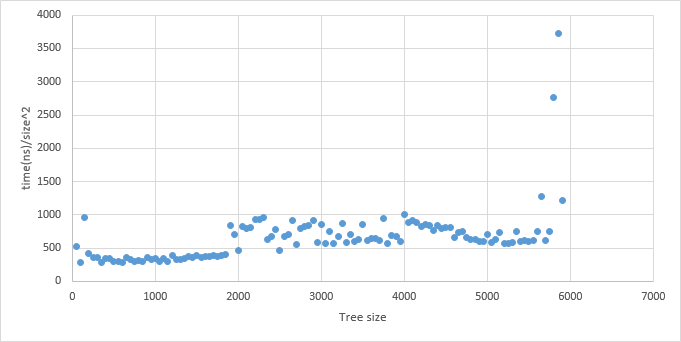
\includegraphics[width=\textwidth]{nsquaredBestCaseTreesTimeDivided}
	\caption{The runtime of the $O(n^2)$ algorithm given trees where each internal node has a leaf as one of its children.}
	\label{nsquaredBestCaseTreesGraph}
	
	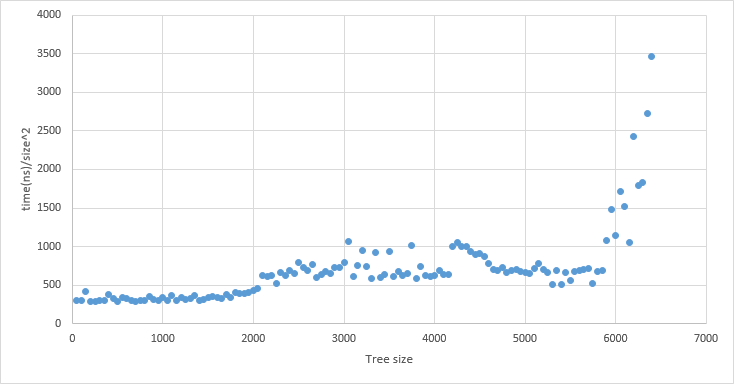
\includegraphics[width=\textwidth]{nsquaredIdenticalCompleteTreesTimeDivided}
	\caption{The runtime of the $O(n^2)$ algorithm given identical complete trees.}
	\label{nsquaredIdenticalCompleteTreesGraph}
\end{figure}

\subsection{Garbage Collecting}
We created a test to measure how much time was used by the garbage collector for each run of the algorithm. We ran the algorithm for the exact same input trees and plotted the runtime of the garbage collector for each tree size. The result is the graph shown in figure \ref{nsquaredGCGraph}. Here we see some of the same behaviour as for the runtime of the algorithm which indicates that the unexpected behaviour was caused by the garbage collector. Figure \ref{nsquaredGCSubtractedGraph} shows a graph where the time used on garbage collecting is subtracted from the time used on running the algorithm. This graph looks more like what we expected of the algorithm. Having divided the runtime by $n^2$, we would expect the graph to stay below some constant. This seems to be the case for a constant of \textasciitilde 600 which suggests that the runtime of the algorithm is indeed $O(n^2)$.

\begin{figure}
	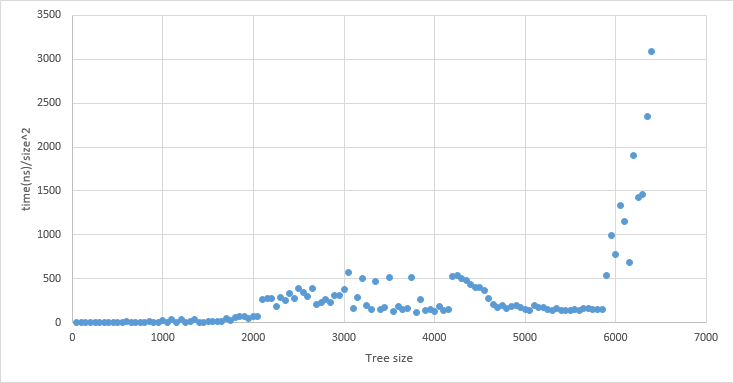
\includegraphics[width=\textwidth]{nsquaredIdenticalCompleteTreesGCTimeDivided}
	\caption{The runtime of the garbage collector when running the $O(n^2)$ algorithm given identical complete trees.}
	\label{nsquaredGCGraph}
\end{figure}

\begin{figure}
	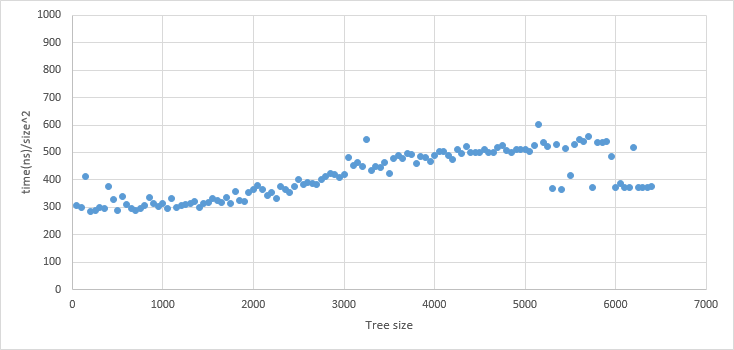
\includegraphics[width=\textwidth]{nsquaredIdenticalCompleteTreesGCSubtractedTimeDivided}
	\caption{The runtime of the $O(n^2)$ algorithm given identical complete trees, after subtracting the runtime of the garbage collector.}
	\label{nsquaredGCSubtractedGraph}
\end{figure}

\section{The $O(nlogn)$ Algorithm}
We know that the runtime of the algorithm by Cole et. al. \cite{nlogn} is $O(nlogn)$ for $n$ sized trees. However, we would like to find out how the algorithm runs in practice. How is the average runtime for random looking trees? What kind of trees give the best runtime? What kind of trees give the worst?

In the following sections we will walk through some of the experiments we did in order to answer these questions.

\subsection{Random Trees}
In practice, an algorithm like this will most likely be used on many very different looking trees. We therefore made an experiment to test how the runtime of the algorithm would look for randomly generated trees.

We ran the algorithm on randomly created trees of sizes $100, 200, ..., 60000$.

The result of this experiment is seen in Figure \ref{randomTreesGraph}. Since we expected the algorithm to have runtime $O(nlogn)$, we divided the runtime with $nlogn$ and the graph should stay below some constant. However, this is not exactly what we see in the graph. There are two things to notice. At size \textasciitilde 5000, \textasciitilde 30000 and \textasciitilde 40000 there is a sudden increase in runtime and from size \textasciitilde 40000 the graph seems to keep increasing. At size \textasciitilde 52000 the JVM ran out of memory which stopped the execution.

\begin{figure}
	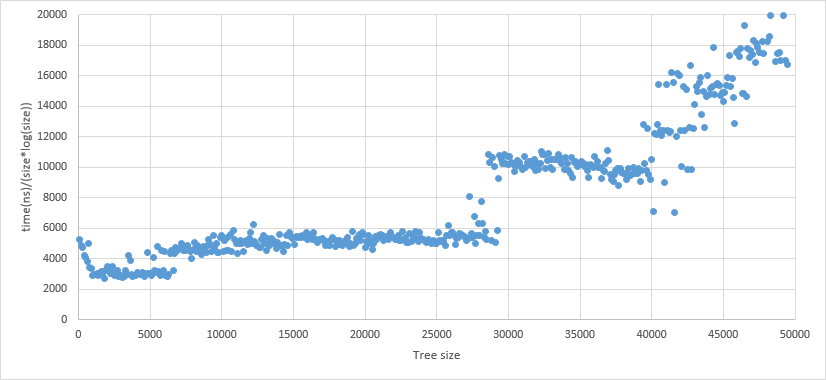
\includegraphics[width=\textwidth]{randomTreesGraph}
	\caption{The runtime of the $nlogn$ algorithm given random trees.}
	\label{randomTreesGraph}
\end{figure}

We suspected this behaviour to be caused by the garbage collector and therefore executed the same experiment again, but this time plotting the runtime of the algorithm after having subtracted the runtime of the garbage collector. The result is shown in figure \ref{randomTreesGCSubtractedGraph} after having divided the runtime with $nlogn$. This graph indeed looks like it will stay below some constant. We therefore believe that the runtime of the algorithm has an upper bound of $O(nlogn)$.

%\begin{figure}
%	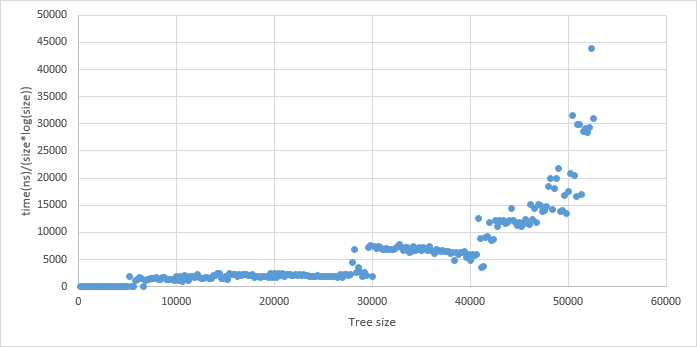
\includegraphics[width=\textwidth]{randomTreesGCGraph}
%	\caption{The runtime of the garbage collector when running the $nlogn$ algorithm given random trees.}
%	\label{randomTreesGCGraph}
%\end{figure}

\begin{figure}
	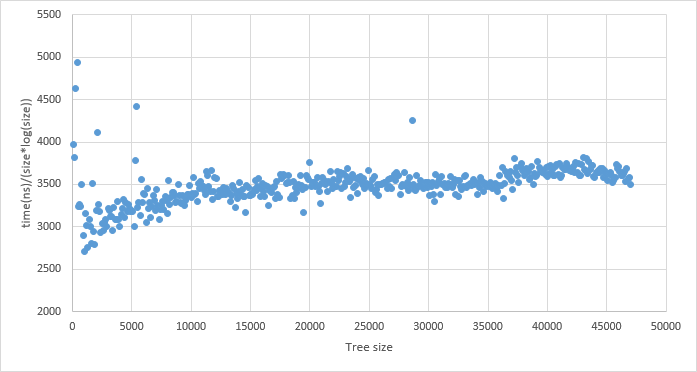
\includegraphics[width=\textwidth]{randomTreesGCSubtractedGraph}
	\caption{The runtime of the $nlogn$ algorithm given random trees after subtracting the time used on garbage collecting.}
	\label{randomTreesGCSubtractedGraph}
\end{figure}

\begin{figure}
	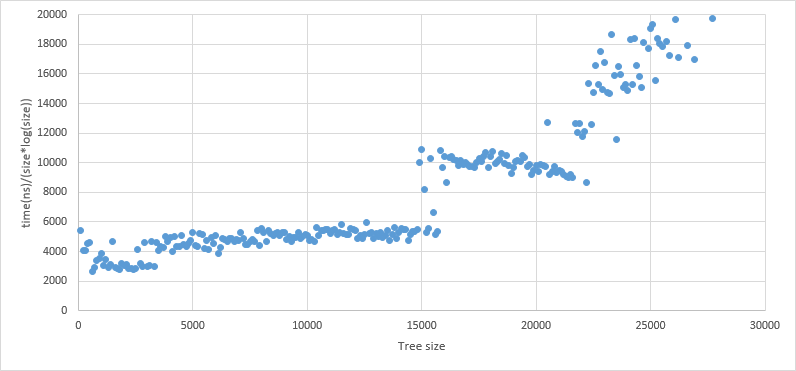
\includegraphics[width=\textwidth]{randomTrees1024MBGraph}
	\caption{The runtime of the $nlogn$ algorithm given random trees with 1024 MB allocated memory.}
	\label{randomTrees1024MBGraph}
\end{figure}

\subsubsection{Behaviour of the Garbage Collector}
We still want to be able to explain this behaviour of the garbage collector, e.g. why the amount of work needed by the garbage collector increases at those exact tree sizes. So we tried running the same experiment again, but with a different amount of allocated memory. In the previous tests, a memory heap of 2048 MB were allocated. In figure \ref{randomTrees1024MBGraph} we see the result of the same experiment, but with a memory heap of 1024 MB allocated. In this experiment, we see the same increases in runtime of the garbage collector, but they happen earlier than in the previous experiment. This indicates that the garbage collector used in these experiments will run depending on how much free memory is left. Using a computer with more RAM so that a larger memory heap can be used could therefore result in a better runtime for large input trees. The algorithm should also be able to work for input trees larger than 50000 when allocating more than 2048 MB of memory.

\subsection{Best Case Trees}
The part of the algorithm that requires most processing power is creating the matching graphs and processing them to compute largest weight agreement matchings. Matching graphs consists of edges and computing LWAMs is done by processing these edges. A tree topology that minimizes the runtime of the algorithm could therefore be a topology that minimizes the number of edges that needs to be created. Since the garbage collector has a large impact on the runtime in practice, it will also make sense to find a tree structure that minimizes the space consumption of the algorithm. The algorithm uses space on storing matching graphs, so minimizing the number of edges that needs to be created seems like a good choice.

Recall how the edges are determined. For each leaf in $T_2$, an edge will be created for each centroid path encountered from the leaf to the root of $T_2$. For any two trees $T_1$ and $T_2$ that are given the algorithm, at least one edge will be created for each leaf of $T_2$ since all leaves will encounter the centroid path starting at the root of $T_2$. The number of edges created will therefore be minimal when $T_2$ has as few centroid paths as possible. Having a tree topology where each internal node has a leaf as one of its children, $T_2$ will have only one centroid path, so only one edge will be added for each leaf in $T_2$.

The process of creating edges is however done in every recursive call of the algorithm, so we want a structure of $T_1$ that gives the fewest possible recursive calls. Choosing the same tree structure as for $T_2$ means that each side tree of $\pi$ will have size 1 so there will be no recursive calls. The result is that the total number of edges created by the algorithm is equal to the number of leaves in $T_2$, namely $n$. This actually means that the step of creating matching graphs in the algorithm only requires $O(n)$ space, instead of $O(nlogn)$.

When processing a matching graph $G(x), x \in X$ to compute LWAMs, each edge $(u_i, v_j)$ will be processed where the leaf in the search tree corresponding to $v_j$ is searched for in $O(log\frac{|T_2(x)|}{n_j})$ time for singleton edges. Having input trees of the topology just mentioned, means that there is only one graph $G(r)$, where $r$ is the root of $T_2$. All edges are singleton edges and for each node $v_j$, $n_j = 1$. So even with this tree topology, the total runtime of the algorithm is $O(\sum_{v_j \in \pi(r)} log |T_2(r)|) = O(nlogn)$. We therefore don't expect an asymptotic improvement of the runtime compared to the result with random trees, but we do expect a noticeable constant improvement.

Another thing about the input trees that affects the runtime of the algorithm, is how similar the two trees are. The more they have in common, the larger the LWAMs will become, and processing these LWAMs will take more time. Since the similarity of the trees does not affect the amount of edges created for this tree structure, the algorithm will be fastest for trees that are not similar. Again we don't expect an asymptotic improvement compared to using identical trees, but a slight constant improvement.

We created an experiment for running the algorithm on trees of the structure explained earlier where the two trees were identical, and one where the leaves in the second tree appeared in the opposite order than that of the first tree.

The graphs in figure \ref{identicalBaseCaseTreesGraph} and \ref{nonidenticalBaseCaseTreesGraph} shows the runtime of the algorithm, using the two kinds of inputs just explained. Comparing the two graphs, it looks like there is actually no significant difference in runtime, so it seems like the size of the LWAMs doesn't affect the runtime of the algorithm much for this kind of input trees. As expected, it looks very much like the algorithm is running in $O(nlogn)$ time, but it is still significantly faster than what we saw for random tree inputs.

\begin{figure}
	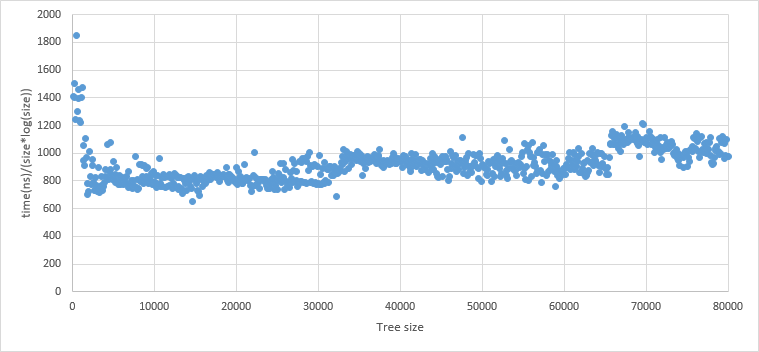
\includegraphics[width=\textwidth]{identicalBaseCaseTreesGraph}
	\caption{The runtime of the $nlogn$ algorithm given two identical best case trees.}
	\label{identicalBaseCaseTreesGraph}
	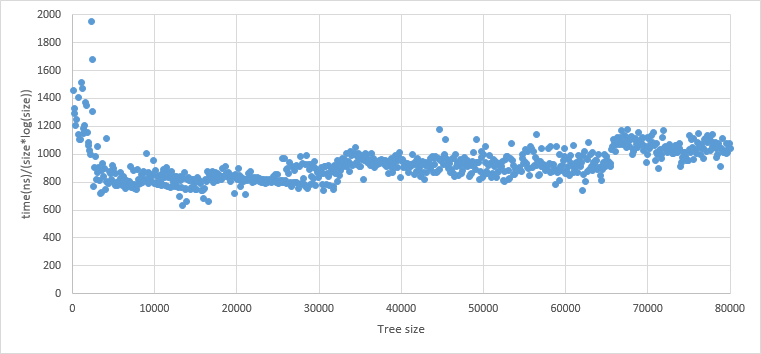
\includegraphics[width=\textwidth]{nonidenticalBaseCaseTreesGraph}
	\caption{The runtime of the $nlogn$ algorithm given two nonidentical best case trees.}
	\label{nonidenticalBaseCaseTreesGraph}
\end{figure}

Another thing to notice is that we don't see the sudden increases in runtime as we did when inputting random trees. This can be due to the fact that less space is used on the matching graph, but also that there are no recursive calls meaning that the program does not use up memory on side trees, induced subtrees etc. Therefore the garbage collector has less work to do.

\subsection{Worst Case Trees}
Since the runtime of the algorithm can be minimized by inputting trees that minimizes the number of edges created, we expect that the input trees that gives the worst runtime are trees that maximizes the number of edges that are created by the algorithm. This should also increase the space consumption.

Again, recall that for each leaf in $T_2$, an edge will be created for each centroid path encountered from the leaf to the root of $T_2$. Now consider the centroid path $\pi(r)$ with nodes $v_1, v_2, ..., v_q$ starting at the root node $r$, where $q \ge 4$. The leaf $v_q$ will encounter only one centroid path on the path to $r$, namely $\pi(r)$ no matter the structure of $T_2$, so a single edge is created. The side tree $N_{q-1}$ is a single leaf. Otherwise $\pi(r)$ would include the root of $N_{q-1}$ instead of $v_q$. That leaf also encounters exactly one graph. The side tree $N_{q-2}$ contains at most 2 leaves or $\pi(r)$ would have included the root of $N_{q-2}$ instead of $v_{q-1}$. If $N_{q-2}$ is a single leaf, it will encounter only one centroid path, but if $N_{q-2}$ contains 2 leaves, both leaves will encounter 2 centroid paths. Continuing this way we can argue that in order to maximize the number of edges created in the algorithm, each side tree of the centroid paths of $T_2$ should hold as many leaves as possible. Creating $T_2$ with this in mind, results in a complete binary tree.

Now let's consider the structure of $T_1$. Since the process of creating edges is done in every recursive call of the algorithm, we want a structure of $T_1$ that results in as many recursive calls as possible with the largest possible trees. A recursive call is made for each side tree of $\pi$, so making these as large as possible will result in the most edges being created. This means that also $T_1$ should be a complete binary tree. Maximizing the amount of recursive calls and the size of the trees in the recursive calls also means that the amount of space needed by the algorithm for these trees is maximized.

To see the runtime of these kind of input trees, we created an experiment for running the algorithm with only complete binary trees as input. We explained earlier that if the input trees are similar, the LWAMs will be larger. However it also means that there will be fewer edges in the matching graphs, since the leaves of a side tree in $T_1$ will be split out over fewer side trees in $T_2$, so that might affect the runtime even more.

The graphs in figure \ref{completeIdenticalTreesGraph} and \ref{completeNonidenticalTreesGraph} shows the result of the experiment when the input trees are identical and when the leaves are randomly distributed in the trees. From these graphs, we see that there is not a significant difference in runtime between the two. In both cases, it is easily seen that the runtime is worse than when inputting random trees, and again we see sudden increases in runtime when reaching certain tree sizes. Already at tree size \textasciitilde 42000, the JVM ran out of memory and could not continue the execution. 
By choosing this tree topology, we tried to maximize the space consumption of the algorithm and the garbage collector therefore needs to run more often and causes the increase in runtime. The graph in figure \ref{completeIdenticalTreesGCSubtractedGraph} shows the runtime of the algorithm after having subtracted the runtime of the garbage collector. As expected, the algorithm still seems to satisfy the runtime upper bound of $O(nlogn)$.

\begin{figure}
	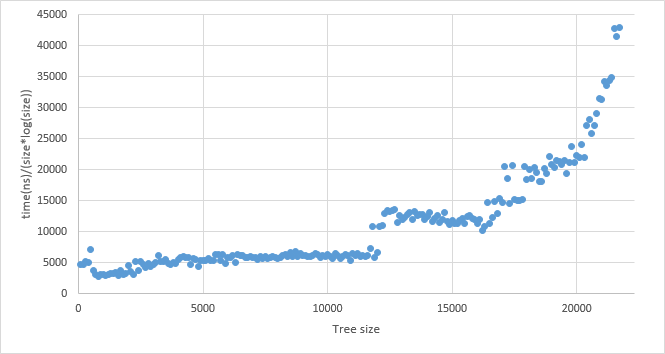
\includegraphics[width=\textwidth]{completeIdenticalTreesGraph}
	\caption{The runtime of the $nlogn$ algorithm given two identical complete trees.}
	\label{completeIdenticalTreesGraph}
\end{figure}
\begin{figure}
	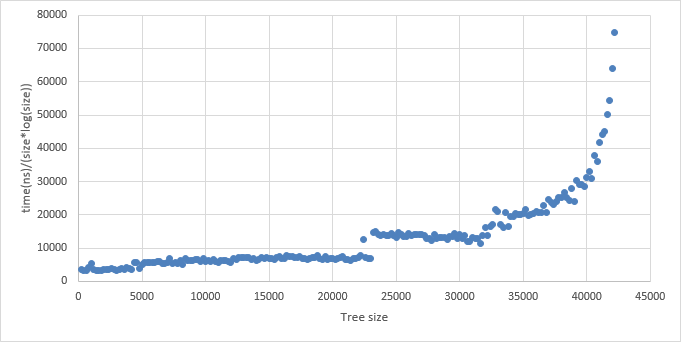
\includegraphics[width=\textwidth]{completeNonidenticalTrees}
	\caption{The runtime of the $nlogn$ algorithm given two nonidentical complete trees.}
	\label{completeNonidenticalTreesGraph}
\end{figure}

%\begin{figure}
%	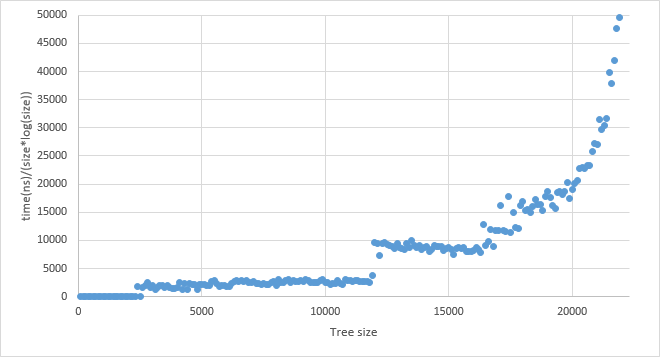
\includegraphics[width=\textwidth]{completeIdenticalTreesGCGraph}
%	\caption{The runtime of the garbage collector when running the $nlogn$ algorithm given two identical complete trees.}
%	\label{completeIdenticalTreesGCGraph}
%\end{figure}
\begin{figure}
	\includegraphics[width=\textwidth]{completeIdenticalTreesGCSubtracted}
	\caption{The runtime of the $O(nlogn)$ algorithm given two identical complete trees after having subtracted the runtime of the garbage collector.}
	\label{completeIdenticalTreesGCSubtractedGraph}
\end{figure}

\section{Comparing Algorithms}
In figure \ref{nsquaredVsNlognGraph} we see the runtime of the two algorithms, given identical complete trees as input. Clearly, there is a huge improvement from the $O(n^2)$ algorithm to the $O(nlogn)$ algorithm and even for small input trees, the $O(nlogn)$ algorithm is dominant. In figure \ref{nsquaredVsNlognSmallTreesGraph}, we can see the difference in runtime for smaller input trees. For input trees of size smaller than \textasciitilde 60, the runtime of the two algorithms are very similar.

\begin{figure}
	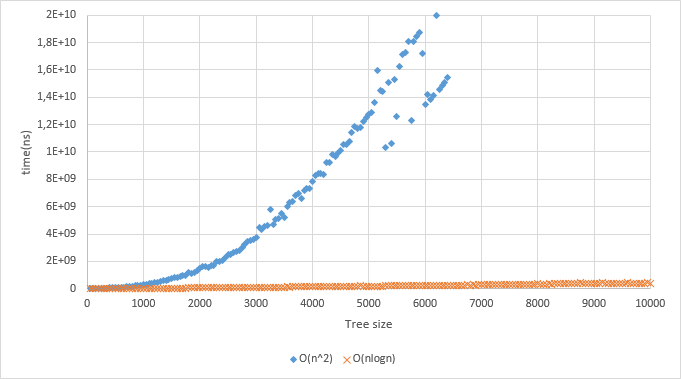
\includegraphics[width=\textwidth]{nsquaredVsNlogn}
	\caption{The runtime of the $O(n^2)$ algorithm and the $O(nlogn)$ algorithm given identical complete trees after having subtracted the runtime of the garbage collector.}
	\label{nsquaredVsNlognGraph}
\end{figure}
\begin{figure}
	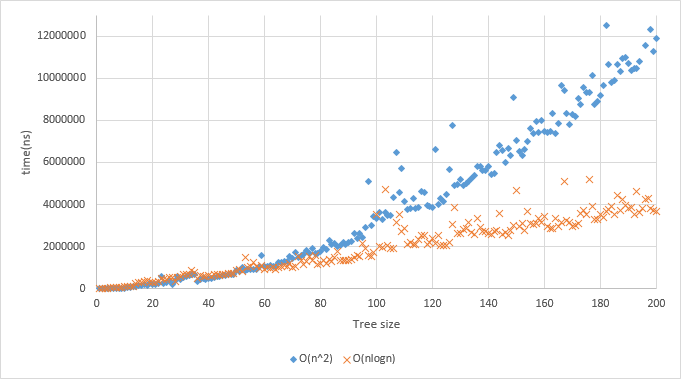
\includegraphics[width=\textwidth]{nsquaredVsNlognSmallTrees}
	\caption{The runtime of the $O(n^2)$ algorithm and the $O(nlogn)$ algorithm given identical complete trees after having subtracted the runtime of the garbage collector.}
	\label{nsquaredVsNlognSmallTreesGraph}
\end{figure}

\section{MLIS}
The small algorithm that we described in section \ref{mlisSection} only works for input trees of a special structure; the same tree structure that we evaluated would give the shortest runtime for the algorithm by Cole et. al. It is expected to run in $O(nlogn)$ time, but because of its simplicity, we expect it to be faster than the algorithm by Cole et. al. in practice. We tested this through an experiment where we ran the two algorithms with the exact same input trees and plotted the results in the graphs seen in figure \ref{baseCaseTreesColeVsLIS}

\begin{figure}
	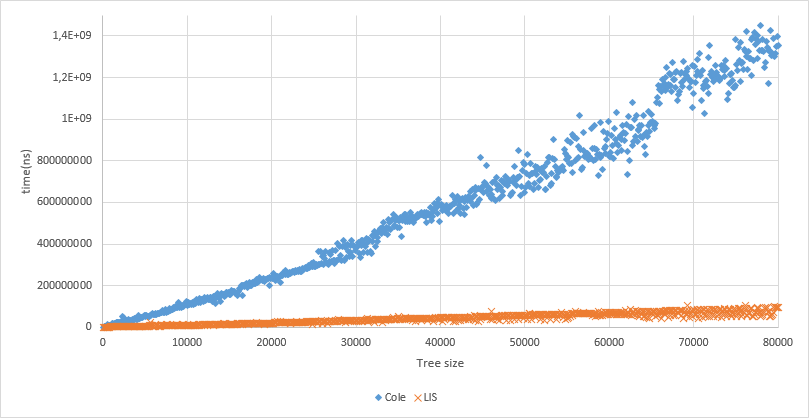
\includegraphics[width=\textwidth]{baseCaseTreesColeVsLIS}
	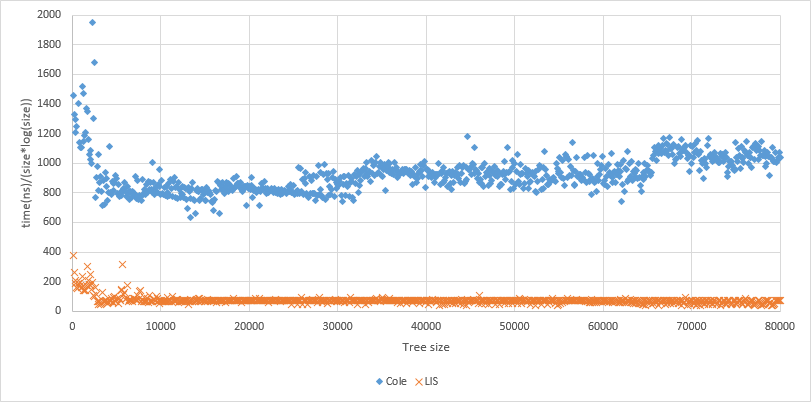
\includegraphics[width=\textwidth]{baseCaseTreesColeVsLISTimeDivided}
	\caption{The runtime of the $nlogn$ algorithm and the algorithm using MLIS given a special type of trees.}
	\label{baseCaseTreesColeVsLIS}
\end{figure}

From the second graph, we conclude that both algorithms satisfy the $O(nlogn)$ runtime and from both graphs it is clear that the algorithm using MLIS has a better runtime.



